\section{Celda Rauch (Deliyannis-Friend modificada)}

\subsection{Introducción}

Se busca mediante el uso de una celda de Rauch o también conocida como Deliyannis-Friend y la aproximación de Chebyshev para diseñar un filtro pasa banda con las siguientes parámetros:

\begin{table}[H]
    \centering
    \resizebox{0.5\textwidth}{!}{%
    \begin{tabular}{cc}
    \hline
    \multicolumn{2}{c}{Par\'ametros de diseño} \\ \hline
    Pendiente de pasabajos normalizado & -40dB/dec \\
    $f_p$ & 64KHz \\
    B & 1/10 \\
    $A_p$ & 3dB \\
    $Z_{in}(f)$ & $\geq 50K\Omega$ \\
    Filtro & Pasa-Banda\\\hline
    \end{tabular}%
    }
    \caption{Par\'ametros de diseño para el filtro a implementar}
    \label{ej22diseno}
\end{table}

Para ello debemos primero introducir la celda de Rauch que tiene la forma:

\begin{figure}[H]
    \centering
    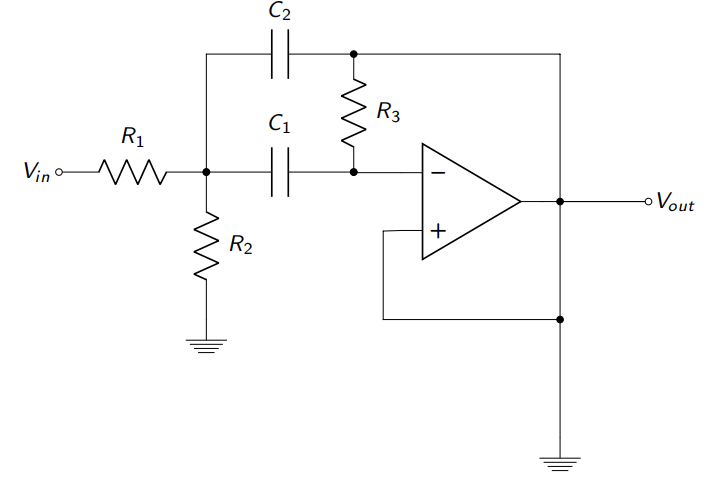
\includegraphics[scale = 0.6]{../Ejercicio2-DisenoDeCeldas/2CELDARAUCH/Informe/circuito3.png}
    \caption{Celda de Rauch}
    \label{ej22cirbasic}
\end{figure}

Sin embargo, se observa que uno de los requisitos que debe cumplir el filtro es que $B = \frac{1}{Q} = \frac{1}{10}$, un valor de Q hace que las relaciones entre las resistencias R1 y R2 sean muy elevados, puesto que los valores de estas resistencias son inversa y directamente proporcionales, respectivamente, a este valor. Es por ello que se utiliza la versión modificada de la la celda Deliyannis-Friend que hace uso de un ciclo de realimentación positiva logrando asi valores elevados de Q.

\begin{figure}[H]
    \centering
    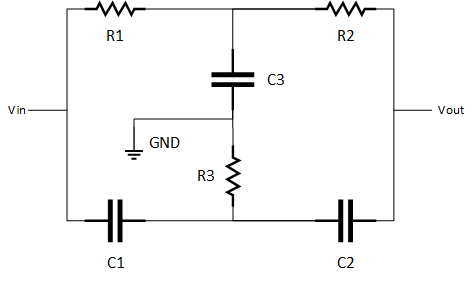
\includegraphics[scale = 0.6]{../Ejercicio2-DisenoDeCeldas/2CELDARAUCH/Informe/circuito.png}
    \caption{Celda de Rauch Mejorada}
    \label{ej22cirbasic}
\end{figure}

Luego analizando el circuito con amplificadores operacionales ideales, o sea los $A_{vol} \longrightarrow \infty$, nos queda que la transferencia de la misma es:
\begin{equation}
    \label{ej22eqh}
    H(s) = \frac{sC2R2R3(RA+RB)}{s^2(C1C2R1R2R3RB) + s(C1R1R2RB + C2(R1R2RB - RA(R1R3 + R2R3))) + RB(R1+R2)}
\end{equation}
Conociendo que las resistencia de retroalimentación valen $RA = KR$ y $RB = (1-K)R$ y si conciderando los capacitores iguales ($C = C1 = C2$) obtenemos que:
\begin{equation}
    \label{ej22eqq}
    Q = \frac{\sqrt{R1R2R3(R1 + R2)}}{2R1R2 - \frac{K}{1 -K} (R1 + R2)R3}
\end{equation}
\begin{equation}
    \label{ej22eqw0}
    \omega_0^2 = \frac{R1+R2}{C^2R1R2R3}
\end{equation}
\begin{equation}
    \label{ej22eqg}
    G = \frac{R2R3}{2R1R2(K - 1) + KR3(R1 + R2)}
\end{equation}

\subsection{Dise\~no del Filtro con Chebyshev}

Para obtener una funci\'on trasferencia que cumpla con una plantilla, es posible utilizar la aproximación\'on de Chebyshev cuyas f\'ormulas caracter\'isticas se muestran en \ref{ej22eqche}.
\begin{equation}
    \begin{split}
        |H(s)|^2 = \frac{1}{1+\epsilon^2 \cdot T_n^2(\omega_N)}, \hspace{0.2cm} \epsilon = \sqrt{10^{\frac{A_p}{10}}-1}
    \end{split}
    \label{ej22eqche}
\end{equation}
Donde $T_n(\omega)$ son los polinomios de Chebyshev.

Debido a que se pide una pendiente de pasa bajos normalizado de $40dB/dec$, el orden de dicho pasa bajos es $n=2$, luego desnormalizando la aproximación, se encuentra que el orden del filtro pasa-banda es 4. En consecuencia, se
utilizarán 2 celdas Rauch de orden 2. Además, se pide una atenuación máxima en banda pasante de $3dB $ pero debido a las tolerancias de los componentes es óptimo una $A_p = 1dB$ para tener margen de error.

Luego, sabiendo que es un filtro pasa-banda podemos establecer la siguiente relación:
\begin{equation}
    \begin{split}
        f_0^2=f_P^+ \cdot f_P^-\\
        B=\frac{\Delta f}{f_0}\\
    \end{split}
    \label{ej22eqb}
\end{equation}

En resumen el filtro tendrá las siguientes propiedades:

\begin{table}[H]
    \centering
    \resizebox{0.4\textwidth}{!}{%
    \begin{tabular}{cc}
    \hline
    \multicolumn{2}{c}{Parámetros de diseño} \\ \hline
    Orden normalizado [n] & 2 \\
    Orden del filtro & 4 \\
    $f_p^+$ & 67kHz \\
    $f_p^-$ & 61kHz \\
    $A_p$ & 1dB \\ \hline
    \end{tabular}%
    }
    \caption{Propiedades del Filtro a Dise\~nar}
    \label{tab:TEMPLATE}
\end{table}

Teniendo en cuenta dichas propiedades, la transferencia del circuito sera:
\begin{equation}
\begin{split}
    H(s) &= \frac{s^2 B^2 \omega_0^2}{s^4+s^3 B \omega_0 1.0977343  + s^2 \omega_0^2 (2+B^2 1.1025103) + s B \omega_0^31.0977343 + \omega_0^4}\\
     &= \frac{ 1.62 \cdot 10^9 s^2}{s^4+ 44.14 \cdot 10^3  s^3 +  3.25 \cdot 10^{11} s^2+  7.13 \cdot 10^{15} s+ 2.61 \cdot10^{22}}
\end{split}
\end{equation}

Como se menciono, utilizaremos dos celdas Rauch en cascada por lo que podemos diseñar el circuito separando la transferencia en dos etapas factorizando, resultando en:
\begin{equation}
    \label{ej22eqhf}
    H(s) = 1.62 \cdot 10^9\frac{s}{s^2 + 21.01\cdot 10^3 s + 1.47 \cdot 10^{11}}\frac{s}{s^2 + 23.13\cdot 10^3 s+ 1.77 \cdot 10^{11}}
\end{equation}

Por otro lado para asegurar que la impedancia de entrada nunca sea menor a $50k\Omega$, se utilizaron 4 amplificadores operacionales. Dos de ellas para el funcionamiento de las celdas, uno se coloco como un buffer entre las dos etapas, asegurando que no se altere ninguna etapa, y el cuarto fue utilizado como buffer de entrada, es decir impedancias muy altas a las frecuencias de interés.


\subsection{Selección de Componentes}

Conociendo entonces la función de transferencia del circuito dado en la ecuación \ref{ej22eqhf} es posible determinar los componentes indicados para el filtro deseado. Estos componentes lo podemos determinar utilizando las siguientes relaciones dado por Schaumann con $Q_0 = 1.5$, el factor óptimo de calidad de la celda Deliyannis-Friend sin mejora, y las respectivas $Q$ y $\omega_0$ del las etapas:

\begin{equation}
\begin{split}
    &Q = \frac{Q_0}{1-2\alpha Q_0^2} \hspace{1.5CM} \alpha = \frac{K}{1-K}\\
    &H_B = \frac{HQ}{Q_0(1-K)} \hspace{1CM}
    R3 = \frac{2Q_0}{\omega_0 C}\\
    &R' = \frac{R3}{4Q_0^2} \hspace{2.3CM}
    a = \frac{H}{2Q_0^2}\\
    &R1 = \frac{R'}{a} \hspace{2.3CM}
    R2 = \frac{R'}{1-a}
\end{split}
\label{ej22eqvalor}
\end{equation}

Despejando desde las ecuaciones \ref{ej22eqvalor} con $C = 1nF$ obtenemos los componentes a utilizar idealmente.

% Please add the following required packages to your document preamble:
% \usepackage{booktabs}
\begin{table}[H]
\centering
\begin{tabular}{@{}ccc@{}}
\toprule
\textbf{Componente}                     & \textbf{Primera Etapa} & \textbf{Segunda Etapa} \\ \midrule
\textbf{C {[}$nF${]}}                     & 1                      & 1                      \\
\textbf{R1 ${[}\Omega{]}$} & 30.11k                 & 27.63k                 \\
\textbf{R2 ${[}\Omega{]}$} & 895.25                 & 815.69                 \\
\textbf{R3 ${[}\Omega{]}$} & 7.82k                  & 7.13k                  \\
\textbf{RA ${[}\Omega{]}$} & 2.03k                  & 2.03k                  \\
\textbf{RB ${[}\Omega{]}$} & 9.97k                  & 9.97k                  \\ \bottomrule
\end{tabular}
\caption{Componentes Ideales}
\label{ej22tvalt}
\end{table}

\subsubsection{Sensibilidad de los Componentes}

Es importante conocer las sensibilidades de los parámetros previo a la selección de componentes, de esta manera tener una idea de que valores pueden variar sin causar grandes cambios en el circuito. 


% Please add the following required packages to your document preamble:
% \usepackage{booktabs}
\begin{table}[H]
\centering
\begin{tabular}{@{}cccc@{}}
\toprule
\textbf{Componentes} & $S_x^w$     & $S_x^H $                                    & $S_x^Q$                                                     \\ \midrule
\textbf{C}           & $-\frac{1}{2}$           & $-\frac{(K-1)R1R2+KR3(R1+R2) }{2R1R2(K-1)+KR3(R1+R2)}$   & $\frac{KR3(R1+R2)}{2(((K-1)2R2+KR3)R1+KR2R3)  }                       $\\
\textbf{R1}          & $-\frac{ R2 }{ 2(R1+R2)}$ & $-\frac{R1(2R2(K-1)+KR3)}{ 2R1R2(K-1)+KR3(R1+R2)}    $    & $-\frac{R2((2R1(K-1)-KR3)R2-KR1R3)}{2(R1+R2)((2R1(K-1)+KR3)R2+KR1R3)} $   \\
\textbf{R2}          & $-\frac{ R1}{2(R1+R2)} $ & $\frac{KR1R3 }{(2R2(K-1)+KR3)R1+KR2R3}  $                 &$-\frac{R1(((K-1)2R2-KR3)R1-KR2R3)}{2(R1+R2)(((K-1)2R2+KR3)R1+KR2R3)}   $ \\
\textbf{R3}          & $-\frac{1}{2}$            &$\frac{2R1R2(K-1)}{(2R2(K-1)+KR3)R1+KR2R3}$               &$\frac{R1((K-1)2R2-KR3)-KR2R3}{2(R1((K-1)2R2+KR3)+KR2R3) }  $            \\
\textbf{K}           &$0 $                &$-\frac{2KR1R2+KR3(R1+R2)}{2R1R2(K-1)+KR3(R1+R2)} $       & $\frac{KR3(R1+R2)}{ (K-1)(R1((K-1)2R2+KR3)+KR2R3)}                 $   \\ \bottomrule
\end{tabular}
\label{ej22tst}
\caption{Ecuaciones de Sensibilidad}
\end{table}

\subsubsection{Selección de Componentes a Utilizar}

Como los valores no suelen ser comerciales se debe adaptar los valores, luego teniendo en cuenta sus sensibilidades se selecciono los componentes a implementar como:

% Please add the following required packages to your document preamble:
% \usepackage{booktabs}
\begin{table}[H]
\centering
\begin{tabular}{@{}ccccc@{}}
\toprule
\textbf{Componente}                     & \textbf{Primera Etapa} & \textbf{Implementación} & \textbf{Segunda Etapa} & \textbf{Implementación} \\ \midrule
\textbf{C {[}nF{]}}                     & 1                      & 1                       & 1                      & 1                       \\
\textbf{R1 ${[}\Omega{]}$} & 30.11k                 & 27k+3k                  & 27.63k                 & 27k+560                 \\
\textbf{R2 ${[}\Omega{]}$} & 895.25                 & 560+330                 & 815.69                 & 560+150+100             \\
\textbf{R3 ${[}\Omega{]}$} & 7.82k                  & 4.7k+3k+100             & 7.13k                  & 6.2k+1k                 \\
\textbf{RA ${[}\Omega{]}$} & 2.03k                  & 2k                      & 2.03k                  & 2k                      \\
\textbf{RB ${[}\Omega{]}$} & 9.97k                  & 10k                     & 9.97k                  & 10k                     \\ \bottomrule
\end{tabular}
\label{ej22tvalr}
\caption{Valores de Componentes Seleccionados}
\end{table}

Luego, realizando un análisis de montecarlo con los componentes utilizados, resistencia de tolerancia $5\%$ y capacitor de tolerancia $20\%$, se obtuvo los posibles casos que enfrentaríamos en una medición experimental.

\begin{figure}[H]
    \centering
    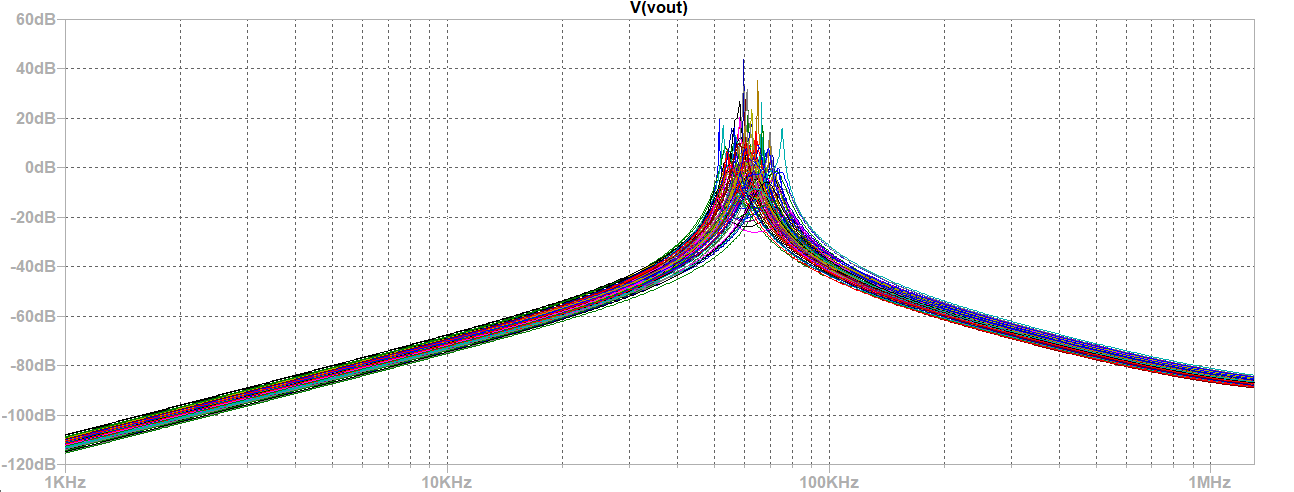
\includegraphics[scale = 0.65]{../Ejercicio2-DisenoDeCeldas/2CELDARAUCH/Informe/monte.PNG}
    \caption{Análisis de Montecarlo}
    \label{ej22monteall}
\end{figure}

Para una representación mas gráfica se realizo un histograma de dispersión por etapa para la verificar del correcto uso de los componentes.

\begin{figure}[H]
    \centering
    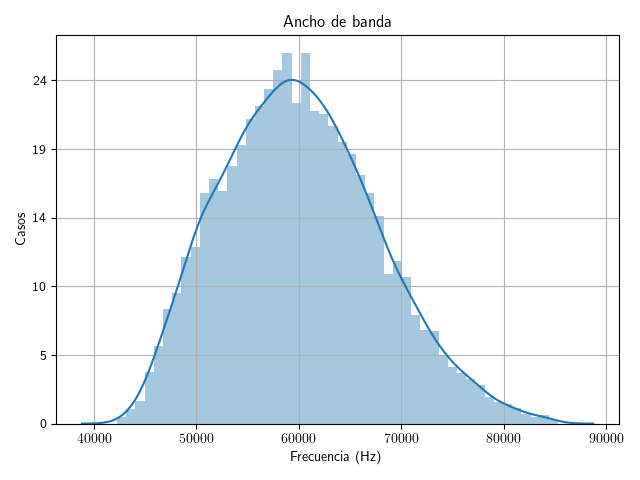
\includegraphics[scale = 0.5]{../Ejercicio2-DisenoDeCeldas/2CELDARAUCH/Informe/disp1.png}
    \caption{Histograma de Dispersión de f0 de la Primera Etapa}
    \label{ej22dis1}
\end{figure}

\begin{figure}[H]
    \centering
    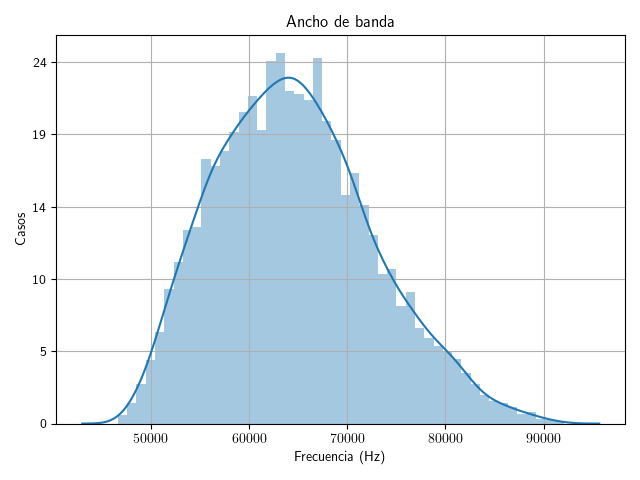
\includegraphics[scale = 0.5]{../Ejercicio2-DisenoDeCeldas/2CELDARAUCH/Informe/disp2.png}
    \caption{Histograma de Dispersión de f0 de la Segunda Etapa}
    \label{ej22dis1}
\end{figure}


\subsection{Análisis de Experimental}

\subsubsection{Respuesta en Frecuencia}

Realizando un análisis en frecuencia, superponiendo resultados teóricos, simulados y experimental se obtuvo el siguiente gráfico:

\begin{figure}[H]
    \centering
    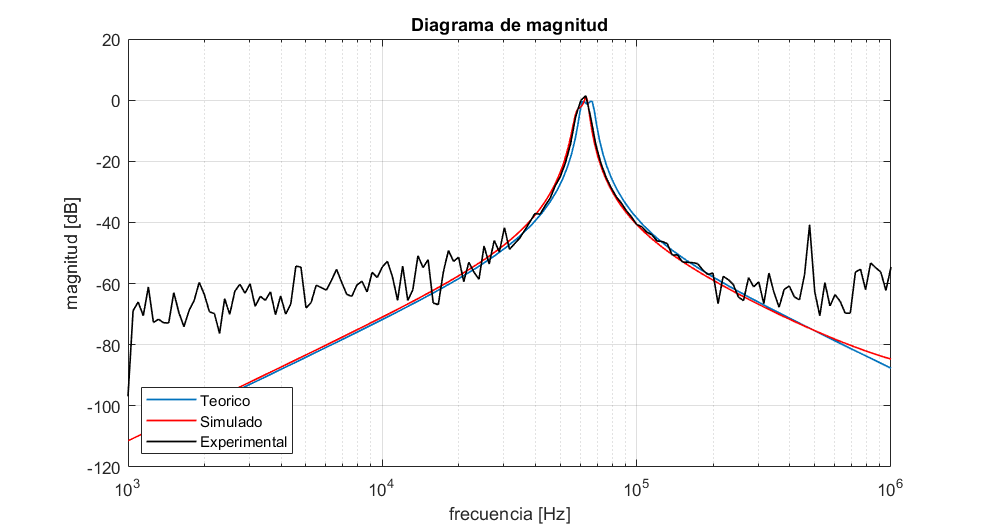
\includegraphics[scale = 0.6]{../Ejercicio2-DisenoDeCeldas/2CELDARAUCH/Informe/bodemag.png}
    % \includegraphics[scale = 0.6]{bodepha.png}
    % \caption{Respuesta en Frecuencia del Circuito}
    % \label{ej22bode}
\end{figure}
\begin{figure}[H]
    \centering
    \includegraphics[scale = 0.6]{../Ejercicio2-DisenoDeCeldas/2CELDARAUCH/Informe/bodepha.png}
    \caption{Respuesta en Frecuencia del Circuito}
    \label{ej22bode}
\end{figure}

En las frecuencias de interés, se puede observarse que se corresponden correctamente los valores medidos con los calculados, si bien con algunas leves diferencias debido a la tolerancia de los componentes pero se encuentra dentro de los resultados esperados. Es importante mencionar que como la atenuación a frecuencias lejanas al $f_0$, el circuito es susceptible al ruido, por lo que las mediciones se verán afectadas grandemente, creando oscilaciones indeseadas. Por otro lado, como se ve en la simulación y en la medición empírica, hay un salto de fase cuando $f>100kHz$, esta alteración es correspondiente al polo inducido por los amplificadores operacionales, dado que ahora no funcionan idealmente. 


\subsubsection{Impedancia de Entrada}

Como los amplificadores operacionales tienen una impedancia de entrada muy elevada, y no tener resistencias comparables para una correcta medición, se estudio la impedancia de entrada desde la simulación.

\begin{figure}[H]
    \centering
    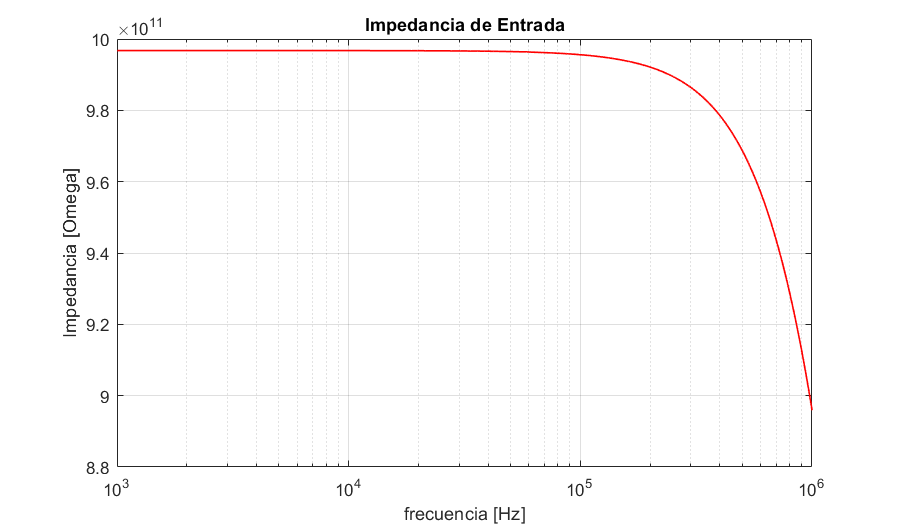
\includegraphics[scale = 0.5]{../Ejercicio2-DisenoDeCeldas/2CELDARAUCH/Informe/zin.png}
    \caption{Impedancia de Entrada Simulado}
    \label{ej22zin}
\end{figure}

\subsubsection{Rango Dinámico}

Para el calculo de rango dinámico, se utiliza la ganancia máxima del circuito experimentado $G = 1.45dB = 1.18$. La tensi\'on m\'axima a la salida ser\'a 6V teniendo en cuenta que la alimentaci\'on $\pm 9V$. Por lo tanto, para hallar la m\'axima tensión sera:

\begin{equation}
    V_i^{MAX} = \frac{V_o^{MAX}}{1.8} = 5.08V
\end{equation}

Luego, suponiendo que la  tensi\'on m\'inima distinguible es el piso de ruido, ya que por debajo de este nivel de tensi\'on no es posible distinguir entre la se\~nal y el ruido, se considera entonces $V_o^{MIN}=10mV$, por lo que resulta que:

\begin{equation}
    V_i^{MIN} = 10mV
\end{equation}

Entonces obtenemos el rango dinámico como:

\begin{equation}
    RD = 20log(\frac{V_i^{MAX}}{V_i^{MIN}})= 54.12dB
\end{equation}

\subsection{Conclusión}

Si bien los resultados resultaron ser similares a la esperado, es indispensable mencionar que no es filtro preciso ya que los componentes utilizados fueron con tolerancias mayores a $5\%$ y no se utilizo prestes debido a la falta de un milímetro para conocer el valor utilizado. Por otro lado, se debe destacar la cualidad de esta celda de Rauch que se pudo obtener un elevado valor de factor de calidad debido a la realimentación positiva y negativa, pero se debe también tener cuidado ya que si los valores del ciclo de realimentación positiva no están bien diseñados, el circuito podría oscilar.


\section{Introducción}

En este apartado se realiza un análisis de la celda denominada Sedra-Ghorab-Martin para posteriormente diseñar, sintetizar y analizar un filtro activo empleando dicha celda con valores recomendados por la cátedra. La principal fuente de información será el paper denominado Optimum configurations for Single-Amplifier Biquadratic Filters.

\section{Celda Sedra-Ghorab-Martin}

La celda Sedra-Ghorab-Martin (en adelante, celda SGB) es un circuito creado en el año 1980 por los miembros de IEEE cuyos nombres se reflejan en el nombre de la celda. Dicho circuito se basa en el circuito pasabanda de Deliyannis, que se reproduce a continuación. Los miembros propusieron dos circuitos bicuadráticos (con funciones transferencia de denominador y numerador de orden dos) que hacen uso del circuito pasabanda de Deliyannis, que se reproduce a continuación:

\begin{figure}[h]
	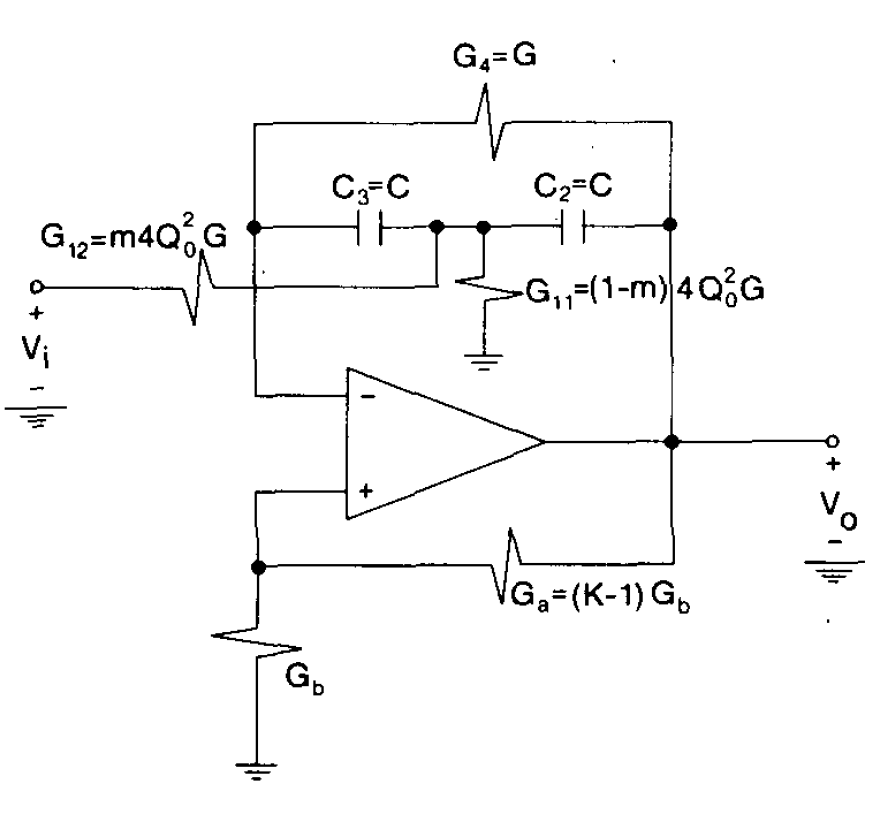
\includegraphics[width=0.8\textwidth]{../Ejercicio2-DisenoDeCeldas/3CeldaSedra/Imagenes/Celda Deliyannis.png}
	\centering
	\caption{Celda Pasabanda de Deliyannis}
	\label{Deliyannis pasabanda}
\end{figure}

Este circuito es posteriormente generalizado por Friend para poder construir cualquier tipo de configuración de filtro. El mismo se caracteriza por poseer una alta selectividad, empleando tanto realimentación positiva como negativa. Sin embargo, para poder sintetizar cualquier tipo de filtro es necesario cargar la red RC que se observa en la realimientación negativa del circuito, lo que hace poco realizable el diseño del mismo. Por otro lado, se encontró que realizando una transformación complementaria sobre el circuito de Deliyannis (esto es, intercambiando la salida del amplificador operacional por masa, y procediendo análogamente con la entrada inversora y no inversora del mismo) se deriva en el circuito de Sallen-Key manteniendo una realimentación positiva. Cabe destacar que esta transformación conserva la sensibilidad de los polos del circuito, pero no así con los ceros de transmisión del mismo. Aún así, se llegó a la conclusión de que es más ventajoso implementar las configuraciones de filtros en una celda Sallen-Key con realimentación positiva (exceptuando el caso de un filtro pasabanda).
En la siguiente figura se muestra como aplicando transformación complementaria y cambios en la red RC se obtienen los distintos circuitos:

\begin{figure}[h]
	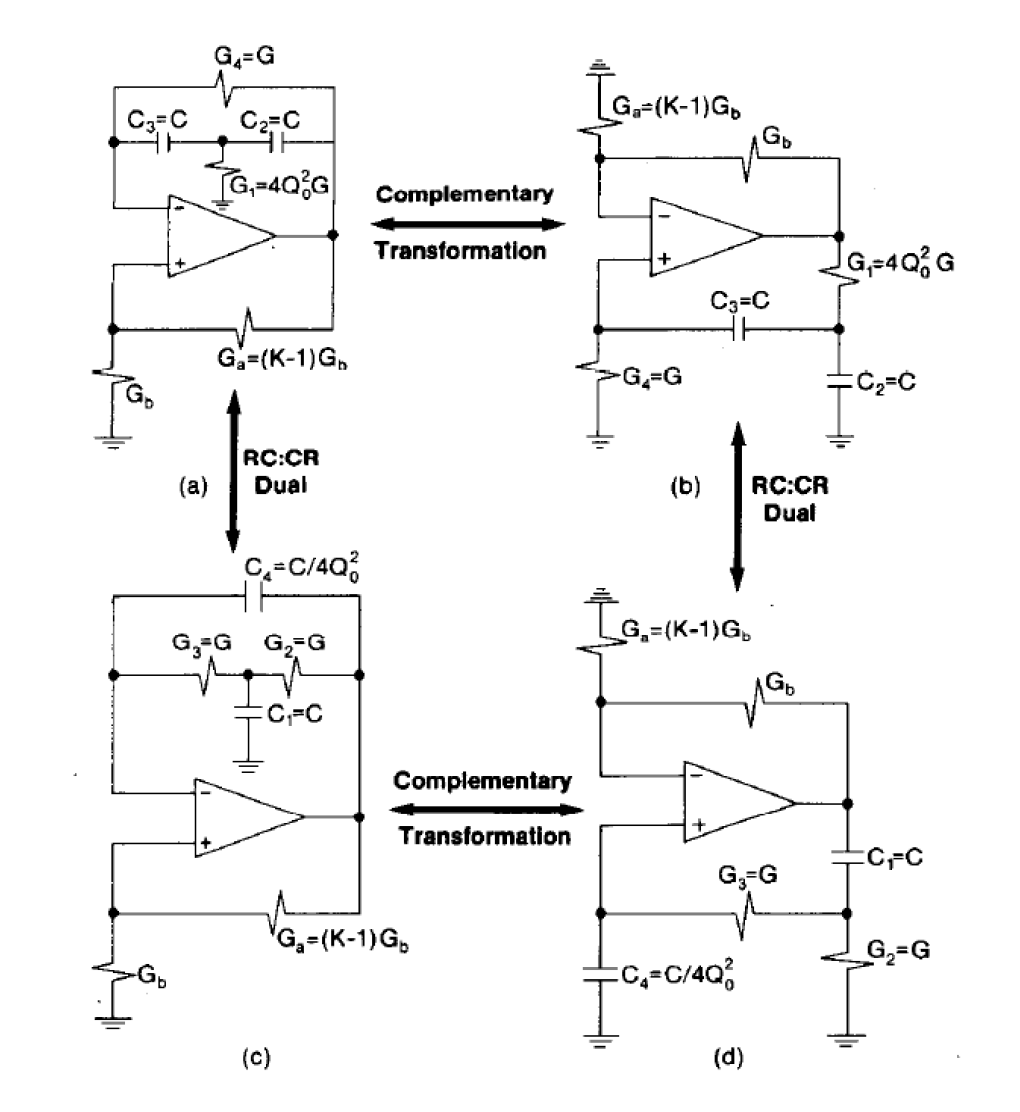
\includegraphics[width=0.8\textwidth]{../Ejercicio2-DisenoDeCeldas/3CeldaSedra/Imagenes/Transformaciones SGB.png}
	\centering
	\caption{Transformaciones de los circuitos }
	\label{transSGM}
\end{figure}

Los circuitos de la figura \ref{transSGM} (b) y \ref{transSGM} (d) son llamados EPF (Enhanced positive feedback), y son la base de la celda SGB. Esta característica esta dada por un coeficiente K $>$ 1. La ecuación que describe el comportamiento de los cuatro circuitos mostrado anteriormente es:

\begin{equation}
	\frac{C}{G} = \frac{2Q_0}{\omega_0}
	\label{eq C/G}
\end{equation}

\begin{equation}
	K - 1 = \frac{1}{2Q_0^2} (1-\frac{Q_0}{Q})
	\label{eq K-1}
\end{equation}

Donde $Q_0$ es un parámetro de diseño que cumple $Q>Q_0$. De esta forma, los circuitos del tipo EPF permiten
implementar filtros con la siguiente función transferencia de segundo orden:

\begin{equation}
	H(s) = \frac{n_2 s^2 + n_1 s + n_0}{s^2 + s (\frac{\omega_0}{Q}) + \omega_0^2}
	\label{eq transferencia general}
\end{equation}

Siendo los coeficientes $n_i$ los ceros de transmision que determinan el tipo de filtro que se implementa. Para poder lograr esto sin afectar la ubicacion de los polos se necesita que aquellos componentes que se encuentren conectados a masa sean desconectados de la misma, total o parcialmente. De esta forma se obtienen los circcuitos HPB(High-Pass Biquad) y LPB(Low-Pass Biquad) que se mostrarán a continuación:

\begin{figure}[h]
	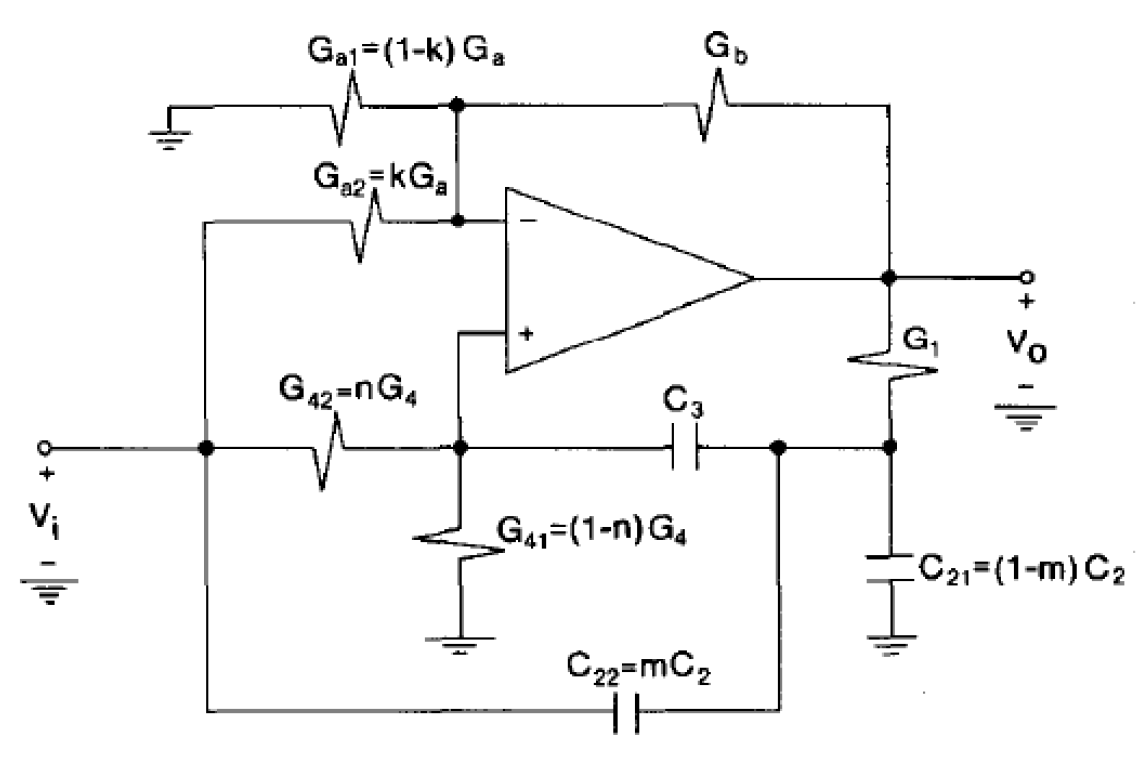
\includegraphics[width=0.6\textwidth]{../Ejercicio2-DisenoDeCeldas/3CeldaSedra/Imagenes/HP biquad.png}
	\centering
	\caption{High-pass biquad}
	\label{HPB}
\end{figure}

\begin{figure}[h]
	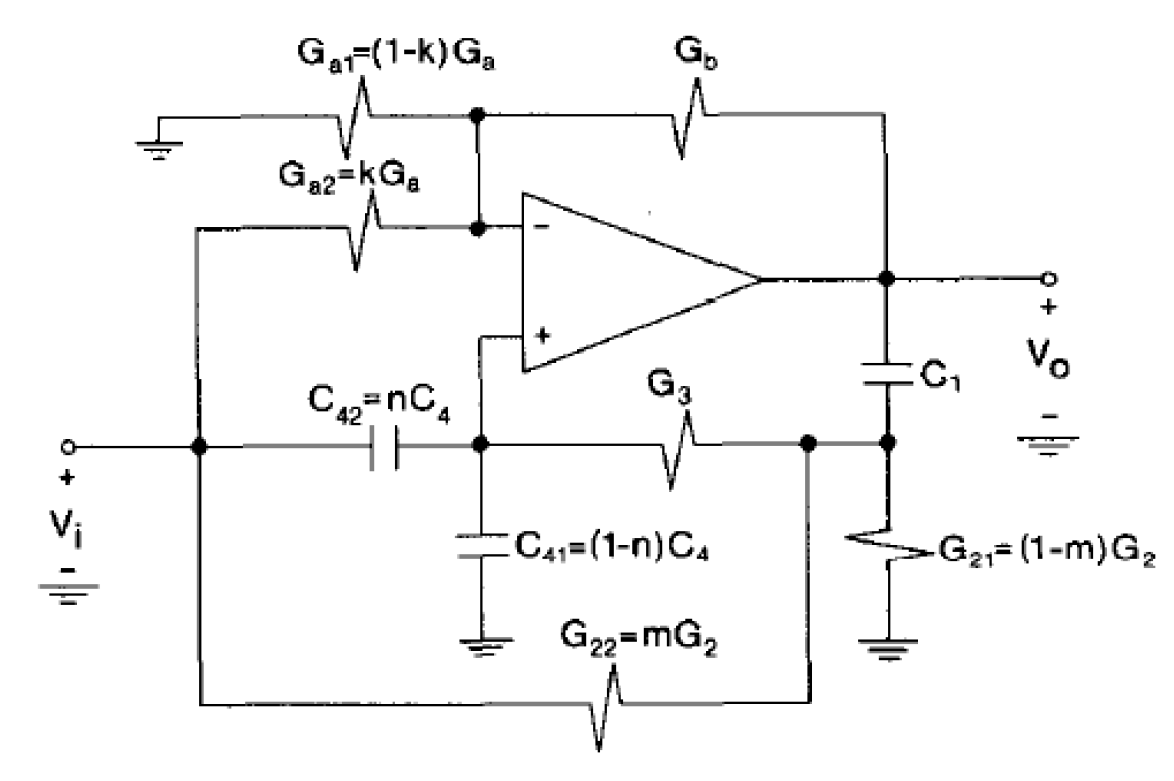
\includegraphics[width=0.6\textwidth]{../Ejercicio2-DisenoDeCeldas/3CeldaSedra/Imagenes/LP biquad.png}
	\centering
	\caption{Low-pass biquad}
	\label{LPB}
\end{figure}

\section{Análisis matemático}

A partir de la ecuacion \ref{eq transferencia general} se puede ver que se deben hallar los coeficientes $n_i$, los cuales están determinados por el tipo de circuito que se desea implementar. En nuestro caso se trata de un HPB por lo que las ecuaciones serán las siguientes:

\subsubsection*{Caso HPB}
\begin{equation}
	n_0= \frac{G_1(G_{41}+G_{42} )}{C_3 ( C_{21} + C_{22} )} \left( \frac{G_{42}}{G_{41}+G_{42}} . \frac{G_{a1}+G_{a2}+G_{b}}{G_b} - \frac{G_{a2}}{G_b} \right)
	\label{coef n0 HPB}
\end{equation}

\begin{equation}
	n_1 = \frac{G_{a1}+G_{a2}+G_b}{G_b} . G_{42}. \left( \frac{1}{C_{21} + C_{22}} + \frac{1}{C_3} \right) - \frac{G_{a2}}{G_b} \left[ \frac{G_1}{C_{21} + C_{22}} + (G_{41}+G_{42}) \left( \frac{1}{C_{21} + C_{22}} + \frac{1}{C_3} \right) \right]
	\label{coef n1 HPB}
\end{equation}

\begin{equation}
	n_2 = \frac{G_{a1}+G_{a2}+G_b}{G_b} . \frac{C_{22}}{C_{21} + C_{22}} - \frac{G_{a2}}{G_b}
	\label{coef n2 HPB}
\end{equation}


\subsubsection*{Caso LPB}

\begin{equation}
	n_0= \frac{G_3(G_{21}+G_{22} )}{C_1 ( C_{41} + C_{42} )} \left( \frac{G_{22}}{G_{21}+G_{22}} . \frac{G_{a1}+G_{a2}+G_{b}}{G_b} - \frac{G_{a2}}{G_b} \right)
	\label{coef n0 LPB}
\end{equation}

\begin{equation}
	n_1 = \frac{G_{a1}+G_{a2}+G_b}{G_b}. G_{42}. \frac{C_{42}}{C_{41}+C_{42}} . \frac{G_{21} + G_{22} + G_3}{C_1} - \frac{G_{a2}}{G_b} . \left( \frac{G_3}{C_{41} + C_{42}} + \frac{G_{21}+G_{22} + G_3}{C_1}\right)
	\label{coef n1 LPB}
\end{equation}

\begin{equation}
	n_2 = \frac{G_{a1}+G_{a2}+G_b}{G_b} . \frac{C_{22}}{C_{21} + C_{22}} - \frac{G_{a2}}{G_b}
	\label{coef n2 LPB}
\end{equation}

En pocas palabras hay que tenes en cuenta los sub-índices en las ecuaciones ya que son complementarias entre si. Para los  denominadores se toman las siguientes ecuaciones características:

\subsubsection*{Caso HPB}

\begin{equation}
\omega_0 = \frac{G_1 ( G_{41} + G_{42} )}{C_3 ( C_{21} + C_{22} ) }
\label{w0 HPB}
\end{equation}

\begin{equation}
\frac{\omega_0}{Q} = (G_{41}+G_{42}). \left( \frac{1}{C_{21} + C_{22}} + \frac{1}{C_3} \right) - \frac{G_1}{C_{21} + C_{22}} . \frac{G_{a1}+G_{a2}}{G_b}
\label{w/Q HPB}
\end{equation}

\subsubsection*{Caso LPB}

\begin{equation}
\omega_0 = \frac{G_3 ( G_{21} + G_{22} )}{C_1 ( C_{41} + C_{42} ) }
\label{w0 LPB}
\end{equation}

\begin{equation}
\frac{\omega_0}{Q} = \frac{G_{21} + G_{22} + G_3}{C_1} - \frac{G_3}{G_{41}+G_{42}} . \frac{G_{a1}+G_{a2}}{G_b}
\label{w/Q LPB}
\end{equation}

\subsection{Sensibilidades}

La sensibilidades del circuito se pueden diferenciar a grandes rasgos por dos muy importantes, las que corresponden a componentes pasivos (resistores y capacitores) y las que corresponden a componentes activos (amplificadores operacionales). El valor de $Q_0$ determina el balance entre los dos tipos de sensibilidades, por lo que su elección debe ser llevada a cabo considerando los valores de dispersión de ambos grupos de componentes. La ecuación que caracteriza $Q_0$ es la siguiente:

\begin{equation}
Q_0 = \left[ |A(s_0)| ^2 . \frac{8\sigma_R^2 + \sigma_C^2}{8\sigma
_A^2} \right] ^\frac{1}{4}
\label{eq Q0}
\end{equation}
Donde $\sigma_R$ es la variación de los resistores, $\sigma_C$ es la variación de los capacitores y $\sigma_A$ es la variación de la ganancia del Op-Amp. Mientras que $A(s_0)$ es la ganancia del amplificador operacional en la frecuencia nominal del polo s0, siendo esta
última:

\begin{equation}
s_0 = -\frac{\omega_0}{2Q} + j\omega_0 \sqrt{1-\frac{1}{4Q^2}}
\label{eq s0}
\end{equation}

A partir de estas ecuaciones es posible determinar las sensibilidades con respecto a cada componente en ambos casos, siendo las sensibilidades correspondientes las mostradas en la siguiente tabla:

\begin{table}[h]
\begin{tabular}{@{}|c|c|c|c|c|c|@{}}
\toprule
\textbf{HPB} & \textbf{$\omega_0$} & \textbf{Q}                         & \textbf{LPB} & \textbf{$\omega_0$} & \textbf{Q}                         \\ 
\midrule
$R_1$         & $-\frac{1}{2}$                      & $-(\frac{Q}{Q_0} - \frac{1}{2})$    & $C_1$         & $-\frac{1}{2}$                      & $-(\frac{Q}{Q_0} - \frac{1}{2})$    \\
$C_2$         & $-\frac{1}{2}$                      & $-\frac{1}{2} (\frac{Q}{Q_0} - 1)$ & $R_2$         & $-\frac{1}{2}$                      & $-\frac{1}{2} (\frac{Q}{Q_0} - 1)$ \\
$C_3$         & $-\frac{1}{2}$                      & $\frac{1}{2} (\frac{Q}{Q_0} - 1)$  & $R_3$          & $-\frac{1}{2}$                      & $\frac{1}{2} (\frac{Q}{Q_0} - 1)$  \\
$R_4$         & $-\frac{1}{2}$                      & $(\frac{Q}{Q_0} - \frac{1}{2})$     & $C_4$         & $-\frac{1}{2}$                      & $(\frac{Q}{Q_0} - \frac{1}{2})$     \\
$R_a$         & 0                                   & $- (\frac{Q}{Q_0} - 1)$            & $R_a$         & 0                                   & $- (\frac{Q}{Q_0} - 1)$            \\
$R_b$         & 0                                   & $ (\frac{Q}{Q_0} - 1)$             & $R_b$         & 0                                   & $ (\frac{Q}{Q_0} - 1)$            
\end{tabular}
\centering
\caption{Tabla de sensibilidades}
\label{tabla sensibilidades}
\end{table}

\subsection{Aproximación del filtro}

La cátedra nos dispuso de una plantilla para implementar un filtro pasa-altos activo. Para tener un margen de tolerancia se usaron valores más restrictivos mostrados en la siguiente tabla:

\begin{table}[h]
\begin{tabular}{@{}|c|c|c|@{}}
\toprule
\textbf{Parámetro} & \textbf{Valor propuesto} & \textbf{Valor elegido} \\ \midrule
$f_a$              & $13,3k\Omega$              & $13,5k\Omega$            \\
$f_p$              & $26,6k\Omega$              & $27k\Omega$              \\
$A_a$              & $40dB$                     & $45dB$      			   \\
$A_p$              & $2dB$                      & $1,5dB$				   \\
$Z_{in}$           & $\geq50k\Omega$            & $\geq50k\Omega$           
\end{tabular}
\centering
\caption{Valores propuesto por la cátedra y elegido por nosotros}
\label{tabla componentes}
\end{table}

El primer paso para el diseño del mismo es normalizar la plantilla a una de un pasa-altos, con frecuencia angular pasante unitaria ($\omega_p =1$). Una vez hecho esto se procede a aplicar la aproximación de Cauer sobre dicha plantilla.
La aproximación de Cauer es una aproximación por funciones elípticas, con riple constante tanto en la banda de paso como la de atenuación. 



\subsection{Etapa I}

\subsection{Etapa II}

